\chapter{Descrizione del Progetto}
\label{cap:descrizione}

Questo capitolo introduce i preliminari tecnici e illustra il problema affrontato. La sezione \ref{Scenario} è dedicata alla descrizione del contesto tecnologico mentre la sezione \ref{Problema} analizza le problematiche affrontate nello studio. 

\section{Scenario Tecnico}
\label{Scenario}

\section{Malware}
Il termine \textbf{malware} deriva dall'unione delle parole inglesi "malicious" e "software" e indica qualsiasi programma o codice progettato per infiltrarsi, danneggiare o ottenere l'accesso non autorizzato a un sistema informatico. I malware possono essere creati con diversi scopi, come il furto di informazioni sensibili, il sabotaggio di sistemi, la visualizzazione di pubblicità indesiderata, o il ricatto delle vittime. Esistono varie tipologie di malware, ognuna con specifiche caratteristiche e metodi di azione.

\subsection{Famiglie di Malware}
Esistono molte famiglie di malware, ognuna con caratteristiche particolari e comportamenti distinti. Tra le più conosciute, possiamo citare:
\begin{itemize}
    \item \textbf{Adware}: Malware progettato per mostrare pubblicità indesiderate sul dispositivo dell'utente, spesso con l'obiettivo di generare guadagni tramite click forzati o visualizzazioni pubblicitarie.
    \item \textbf{Backdoor}: Un tipo di malware che consente l'accesso remoto non autorizzato a un sistema, permettendo all'attaccante di controllare il dispositivo senza che l'utente ne sia a conoscenza.
    \item \textbf{Downloader}: Malware progettato per scaricare e installare altri malware su un dispositivo infetto. Agisce come un "ponte" per introdurre ulteriori minacce nel sistema.
    \item \textbf{Ransomware}: Malware progettato per criptare i dati dell'utente e richiedere un riscatto per la decrittazione. Spesso utilizza tecniche di estorsione per costringere le vittime a pagare somme di denaro in criptovalute.
    \item \textbf{Spyware}: Malware progettato per raccogliere informazioni sull'utente senza il suo consenso, come dati personali, cronologia di navigazione e credenziali, per poi inviarle all'attaccante.
    \item \textbf{Trojan (Cavalli di Troia)}: Programmi che si mascherano come software legittimi per ingannare gli utenti e indurli a installarli. Una volta installati, possono dare accesso al sistema o danneggiarlo.
    \item \textbf{Virus}: Software che si replica infettando altri file eseguibili, spesso con l'intento di danneggiare il sistema o rubare informazioni.
    \item \textbf{Worms}: Simili ai virus, ma non necessitano di un file host per propagarsi. Possono diffondersi autonomamente attraverso la rete, sfruttando vulnerabilità di sicurezza.
    \item \textbf{Rootkit}: Malware progettato per nascondere la presenza di altri malware o del proprio codice su un sistema, integrandosi profondamente nel sistema operativo e rendendosi quasi invisibile agli strumenti di rilevamento tradizionali.
    \item \textbf{Keylogger}: Un tipo di malware che registra ogni battitura dell'utente su tastiera per rubare informazioni sensibili come password e credenziali di accesso.
    \item \textbf{Botnet}: Una rete di dispositivi infetti che possono essere controllati a distanza per compiere azioni malevole, come attacchi DDoS e spam.
    \item \textbf{Fileless Malware}: Malware che non scrive alcun file sul disco, utilizzando invece la memoria e strumenti già esistenti nel sistema operativo, rendendo più difficile la rilevazione.
    \item \textbf{Scareware}: Malware che inganna l'utente facendogli credere che il sistema sia infettato per indurlo a comprare software falsi o fornire informazioni personali.
    \item \textbf{RAT (Remote Access Trojan)}: Trojan che permette all'attaccante di ottenere accesso remoto e controllo completo del dispositivo infetto, consentendo di spiare l'utente e rubare informazioni.
    \item \textbf{Malvertising}: Uso di annunci pubblicitari legittimi per distribuire malware, spesso sfruttando reti pubblicitarie per diffondere link malevoli.
    \item \textbf{Cryptojacker}: Malware che utilizza le risorse di calcolo della vittima per effettuare il mining di criptovalute senza che l'utente ne sia consapevole.
    \item \textbf{Logic Bomb}: Malware che rimane inattivo fino a quando non viene attivato da un evento specifico, come una data o una certa condizione, per poi eseguire azioni malevole come cancellare file o causare crash del sistema.
\end{itemize}

\subsection{Struttura del malware}
Il malware, ovvero software malevolo, presenta una struttura complessa progettata per danneggiare, disturbare o accedere a sistemi informatici senza autorizzazione. La struttura tipica di un malware può includere i seguenti componenti, che variano in base alla famiglia a cui appartiene:
\begin{itemize}
    \item \textbf{Adware}: Include componenti per il monitoraggio delle abitudini di navigazione dell'utente, e un motore per la visualizzazione automatica di annunci pubblicitari.
    \item \textbf{Backdoor}: Contiene un modulo che consente l'accesso remoto non autorizzato, spesso implementato tramite una comunicazione criptata con il server di controllo dell'attaccante.
    \item \textbf{Downloader}: Dispone di un componente per contattare server remoti e scaricare ulteriori malware, spesso utilizzando tecniche di offuscamento per eludere la rilevazione.
    \item \textbf{Ransomware}: Presenta un sistema di criptazione che rende inaccessibili i dati dell'utente, accompagnato da un modulo che mostra un messaggio di riscatto e gestisce i pagamenti.
    \item \textbf{Spyware}: Ha moduli per il keylogging, il monitoraggio della cronologia di navigazione e la raccolta di credenziali, inviando poi queste informazioni agli attaccanti.
    \item \textbf{Trojan}: Include un componente di mimetizzazione, spesso mascherandosi da software legittimo, e può implementare diversi payload per danneggiare il sistema o esfiltrare dati.
    \item \textbf{Virus}: Contiene un modulo di replicazione che gli consente di infettare altri file eseguibili, spesso con funzionalità aggiuntive per danneggiare il sistema.
    \item \textbf{Worms}: Dispone di un motore di propagazione automatica, che sfrutta vulnerabilità note per diffondersi in modo autonomo tra i dispositivi connessi in rete.
    \item \textbf{Rootkit}: Include un modulo per nascondere la presenza del malware all'interno del sistema, modificando componenti del kernel o altri elementi critici del sistema operativo.
    \item \textbf{Keylogger}: Dispone di un modulo per catturare tutte le battiture dell'utente, salvandole in un file log da inviare all'attaccante.
    \item \textbf{Botnet}: Include componenti che consentono di trasformare il dispositivo in un "bot" controllato da remoto, spesso senza che l'utente ne sia consapevole.
    \item \textbf{Fileless Malware}: Utilizza strumenti nativi del sistema operativo (come PowerShell o WMI) per eseguire codice dannoso direttamente in memoria, rendendo più difficile la sua rilevazione.
    \item \textbf{Scareware}: Contiene un modulo per la visualizzazione di avvisi falsi che spingono l'utente ad acquistare software non necessario o dannoso.
    \item \textbf{RAT (Remote Access Trojan)}: Include strumenti per il controllo remoto, consentendo all'attaccante di navigare tra i file, attivare la webcam e installare altri malware.
    \item \textbf{Malvertising}: Contiene codice che viene iniettato tramite banner pubblicitari, spesso sfruttando vulnerabilità del browser per compromettere il sistema dell'utente.
    \item \textbf{Cryptojacker}: Include script di mining che si attivano all'insaputa dell'utente per utilizzare risorse di CPU e GPU per minare criptovalute.
    \item \textbf{Logic Bomb}: Include una condizione preimpostata (come una data specifica o un certo evento) che, una volta soddisfatta, attiva il payload dannoso.
\end{itemize}

\subsection{Dataset}
Nell'ambito di questo progetto di ricerca sono state prese in considerazione solo le prime 7 famiglie di malware, in quanto le più comuni e pericolose. Per la raccolta del dataset sono stati utilizzati campioni di malware provenienti da diverse fonti, tra cui:
\begin{itemize}
    \item \textbf{MalwareBazaar}: Un database di malware che raccoglie campioni da varie fonti e li mette a disposizione della comunità per la ricerca e l'analisi.
    \item \textbf{MalShare}: Un database di malware che raccoglie campioni da varie fonti e li mette a disposizione della comunità per la ricerca e l'analisi.
    \item \textbf{VirusShare}: Un archivio di malware che raccoglie campioni da varie fonti e li archivia per scopi di ricerca e analisi.
\end{itemize}

Per la classificazione dei campioni di malware sono stati utilizzati diversi strumenti di analisi statica e dinamica, tra cui:
\begin{itemize}
    \item \textbf{Virustotal}: Un servizio di scansione malware online che analizza gli eseguibili passati e genera un report in formato JSON contenente le analisi che i vari antivirus hanno effettuato.
    \item \textbf{AVClass2}: Uno strumento di classificazione di malware che etichetta i campioni in base alle famiglie di malware.
    \item \textbf{Ghidra}: Un decompilatore e framework di reverse engineering sviluppato dalla National Security Agency (NSA) degli Stati Uniti.
\end{itemize}

\vspace{.5cm}
Il dataset risultante è composto come segue:

\begin{table}[h]
    \centering
    \begin{tabular}{|l|l|}
        \hline
        \textbf{Famiglia di Malware} & \textbf{Numero di Campioni} \\
        \hline
        Adware & 4566 \\
        Backdoor & 1270 \\
        Downloader & 1128 \\
        Ransomware & 2529 \\
        Spyware & 502 \\
        Trojan & 4058 \\
        Virus & 2061 \\
        \hline
    \end{tabular}
    \caption{Dataset di Malware}
\end{table}


\begin{center}
	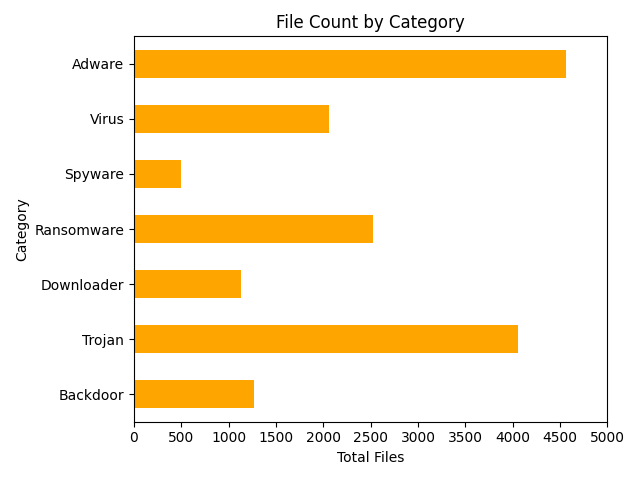
\includegraphics[width=0.7\textwidth]{images/total_families.png}
	\captionof{figure}{Malware families}
\end{center}

% \subsection{Codice usato per la classificazione dei malware}
% \begin{lstlisting}[caption={Codice Python per la generazione del report in formato JSON da VirusTotal},captionpos=b]
% # Codice per generare il report
% import os
% import requests
% import json
% import hashlib
% import time
% from tqdm import tqdm

% from dotenv import load_dotenv

% load_dotenv('variables.env')

% API_KEY = os.getenv('YOUR_API_KEY')
% MALWARE_DATASET_DIR = '../Malware/malware_dataset_virushare_2024/'
% REPORT_DIR = 'report_virushare'
% REQUEST_DELAY = 20  
% INITIAL_DELAY = 30  
% MAX_RETRIES = 3  
% MAX_REPORTS = 500  

% def get_file_hash(file_path):
%     hasher = hashlib.sha256()
%     try:
%         with open(file_path, 'rb') as f:
%             buf = f.read()
%             hasher.update(buf)
%     except Exception as e:
%         print(f"Errore: Impossibile leggere il file {file_path}.")
%         print(e)
%         return None
%     return hasher.hexdigest()

% def upload_file_to_virus_total(file_path):
%     url = 'https://www.virustotal.com/vtapi/v2/file/scan'
%     params = {'apikey': API_KEY}
%     with open(file_path, 'rb') as f:
%         file_data = f.read()
%     files = {'file': (os.path.basename(file_path), file_data)}
%     total_size = len(file_data)
%     with tqdm(total=total_size, unit='B', unit_scale=True, desc='Caricamento') as tqdm_bar:
%         try:
%             response = requests.post(url, files=files, params=params, timeout=20)
%             tqdm_bar.update(total_size)
%             if response.status_code == 200:
%                 print(response.json())
%                 return response.json().get('resource')
%             else:
%                 print(f"Errore nel caricamento del file {file_path}: {response.status_code}")
%                 print(f"Contenuto della risposta: {response.text}")
%                 return None
%         except requests.exceptions.RequestException as e:
%             print(f"Errore nel caricamento del file {file_path}: {e}")
%             return None

% def check_existing_report(file_hash):
%     url = 'https://www.virustotal.com/vtapi/v2/file/report'
%     params = {'apikey': API_KEY, 'resource': file_hash}
%     response = requests.get(url, params=params)
%     if response.status_code == 200:
%         data = response.json()
%         if data.get('response_code') == 1:  
%             return data
%     return None

% def generate_reports():
%     if not os.path.exists(REPORT_DIR):
%         os.makedirs(REPORT_DIR)
    
%     report_count = 0
%     for file_name in os.listdir(MALWARE_DATASET_DIR):
%         if report_count >= MAX_REPORTS:
%             break
        
%         file_path = os.path.join(MALWARE_DATASET_DIR, file_name)
%         if os.path.isfile(file_path):
%             report_path = os.path.join(REPORT_DIR, file_name.replace(" ", "") + ".json")
%             if os.path.exists(report_path):
%                 print(f"Report gia' esistente per {file_name}. Skipping...")
%                 continue
            
%             file_hash = get_file_hash(file_path)
%             if file_hash:
%                 report = check_existing_report(file_hash)
%                 if report:
%                     with open(report_path, 'w') as report_file:
%                         json.dump(report, report_file, indent=4)
%                     report_count += 1
%                     continue
                
%                 resource = upload_file_to_virus_total(file_path)
%                 if resource:
%                     time.sleep(INITIAL_DELAY)  
%                     report = check_existing_report(resource)
%                     if report:
%                         with open(report_path, 'w') as report_file:
%                             json.dump(report, report_file, indent=4)
%                         report_count += 1
%                         print(f"Report generato per {file_name}")

% if __name__ == '__main__':
%     generate_reports()
% \end{lstlisting}

\subsection{Decompilatore}
Nonostante siano disponibili numerose tipologie di decompilatori, in questo progetto si è scelto l'utilizzo di \textbf{Ghidra} in quanto open source, già utilizzato in precedenza e compatibili con architettura arm presente nella macchina utilizzata durante tutto il tempo di svolgimento del progetto. È uno strumento di analisi di software, principalmente noto come un potente decompilatore e framework per il reverse engineering, sviluppato e distribuito gratuitamente dalla National Security Agency (NSA) degli Stati Uniti. Il suo utilizzo in questo progetto consiste in:
\begin{itemize}
    \item decompilazione del codice eseguibile in \textbf{codice assembly} su cui poter effettuare analisi statica. 
    \item Estrazione del codice esadecimale.
\end{itemize}

% \begin{lstlisting}[caption={Codice Python per la decompilazione di malware con Ghidra},captionpos=b]
% import os
% import subprocess
% import tempfile

% def run_ghidra_decompilation(file_path, temp_project_path, output_dir):
%     # Configura i percorsi necessari
%     ghidra_path = "path/to/ghidra_9.2.2_PUBLIC"
%     analyze_headless = os.path.join(ghidra_path, "support/analyzeHeadless")
%     script_path = os.path.join(ghidra_path, "Ghidra/Features/Decompiler/ghidra_scripts")
    
%     # Determina i nomi base del file
%     file_base_name = os.path.basename(file_path)
%     log_file_path = os.path.join(output_dir, f"{file_base_name}_ghidra.log")
    
%     # Output per l'assembly di questo eseguibile
%     assembly_output_path = os.path.join(output_dir, f"{file_base_name}_assembly.txt")

%     # Costruisce il comando
%     command = [
%         analyze_headless,
%         temp_project_path, "tempProject", "-import", file_path,
%         "-postScript", "DecompileAllFunctions.py", assembly_output_path,
%         "-scriptPath", script_path,
%         "-processor", "x86:LE:64:default",
%     ]

%     # Esegue il comando
%     try:
%         subprocess.check_call(command)
%         print(f"Decompilazione completata con successo per il file: {file_path}")
%     except subprocess.CalledProcessError as e:
%         print("Errore durante la decompilazione:", str(e))
%         return

%     if os.path.exists(assembly_output_path):
%         print(f"File assembly salvato in: {assembly_output_path}")
%     else:
%         print(f"File assembly non trovato: {assembly_output_path}")

% def process_all_files(directory, output_dir):
%     assembly_dir = "/path/to/assembly/files"
%     for root, dirs, files in os.walk(directory):
%         for file_name in files:
%             file_path = os.path.join(root, file_name)
%             if os.path.isfile(file_path):
%                 base_name = os.path.splitext(file_name)[0]
%                 txt_file_path = os.path.join(assembly_dir, f"{base_name}_assembly.txt")
%                 if os.path.exists(txt_file_path):
%                     print(f"File assembly gia' esistente per: {file_path}")
%                     continue
%                 with tempfile.TemporaryDirectory() as temp_project_path:
%                     print(f"Processing file: {file_path}")
%                     run_ghidra_decompilation(file_path, temp_project_path, output_dir)

% if __name__ == "__main__":
%     malware_directory = "/path/to/malware/directory"
%     output_dir = "/path/to/output/directory"
%     process_all_files(malware_directory, output_dir)
% \end{lstlisting}

\section{Convolutional Neural Network}
L'architettura della rete neurale convoluzionale (CNN) utilizzata in questo progetto è composta da diversi strati, ciascuno con un ruolo specifico nel processo di apprendimento:
\begin{enumerate}
    \item \textbf{Strati Convoluzionali (Conv2D)}:
    La rete inizia con tre strati convoluzionali, che sono responsabili dell'estrazione delle caratteristiche principali dalle immagini di input in scala di grigi (16x16 pixel).
    Primo strato convoluzionale: utilizza da 32 a 128 filtri (incremento di 32) con kernel di dimensione (3x3). Questo strato mantiene l'input della stessa dimensione (16x16) grazie al padding "same" e utilizza l'attivazione ReLU (Rectified Linear Unit).
    Secondo strato convoluzionale: utilizza da 32 a 64 filtri (incremento di 32) con kernel (3x3) e l'attivazione ReLU, seguito da un'operazione di MaxPooling2D con finestra (2x2), riducendo così la dimensione a (8x8).
    Terzo strato convoluzionale: impiega lo stesso numero di filtri (32-64, incremento di 32) e kernel, con un'ulteriore riduzione dimensionale tramite MaxPooling2D, portando la dimensione finale a (2x2).
    \item \textbf{Strato di Pooling (MaxPooling2D)}:
    Gli strati di pooling riducono la dimensione spaziale delle feature map mantenendo solo le informazioni più rilevanti, riducendo il numero di parametri e migliorando l'efficienza computazionale.
    Sono utilizzati dopo ogni strato convoluzionale con finestre di dimensione (2x2).
    \item \textbf{Strato di Flattening}:
    Dopo la fase convoluzionale, le feature map tridimensionali vengono "appiattite" in un vettore unidimensionale per poter essere processate dagli strati completamente connessi.
    \item \textbf{Strato Completamente Connesso (Dense)}:
    Lo strato completamente connesso riceve l'input dallo strato di flattening. Qui, i neuroni collegano ogni unità precedente a quelle successive, consentendo alla rete di apprendere pattern complessi e interazioni tra le caratteristiche estratte.
    La dimensione del layer è variabile tra 32 e 128 unità, con attivazione ReLU. È anche presente un layer di Dropout, utilizzato per prevenire l'overfitting con un valore di dropout che può variare tra 0.0 e 0.5 (incremento di 0.1).
    \item \textbf{Strato di Output (Dense)}:
    Lo strato finale è un layer completamente connesso con un numero di neuroni pari al numero di classi di malware presenti nel dataset, con attivazione Softmax per ottenere una probabilità normalizzata per ciascuna classe.
\end{enumerate}

\begin{figure}[ht]
    \centering
        \centering
        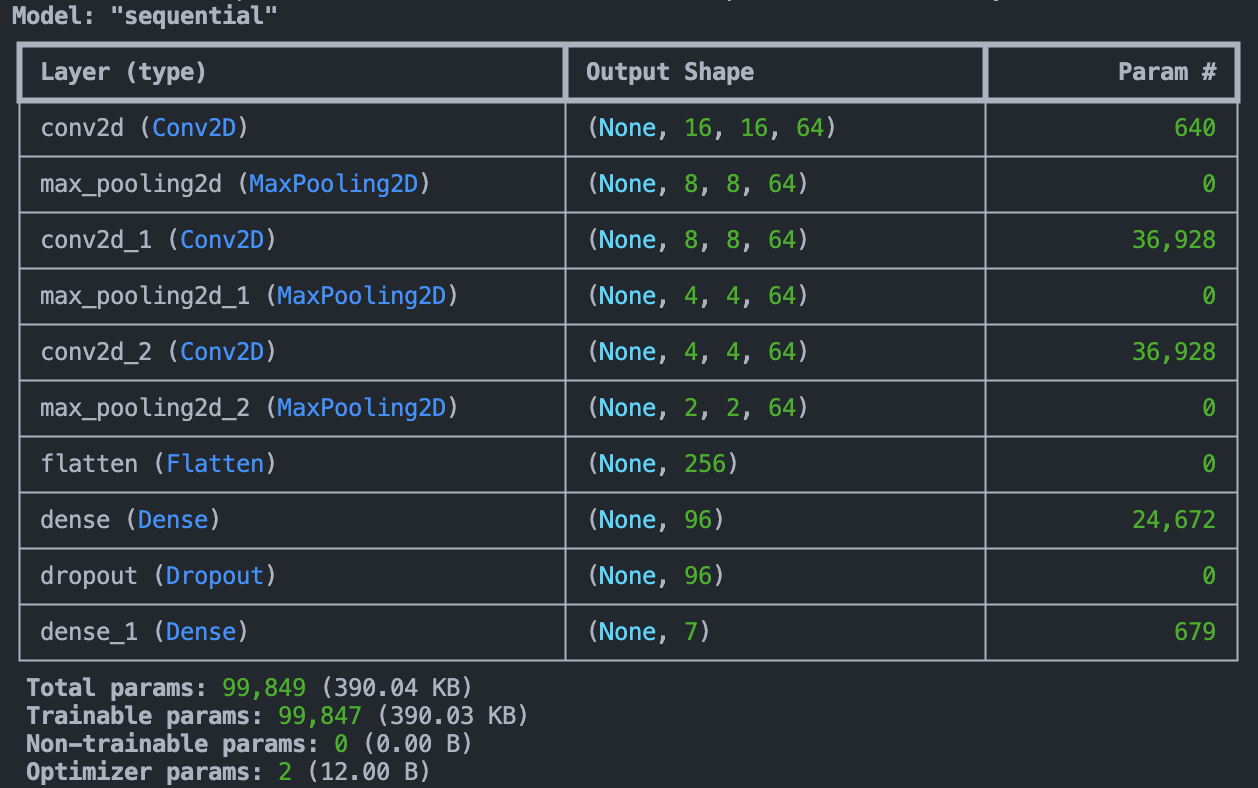
\includegraphics[width=0.8\linewidth]{images/cnn_architecture.png}
        \label{fig:cnn_architecture}
\end{figure}
\captionof{figure}{Architettura della rete neurale convoluzionale (CNN) utilizzata}

\subsection{Addestramento}

\subsection{Metriche di Valutazione del Modello}

Nel campo della classificazione, specialmente in scenari complessi come la classificazione del malware, è importante analizzare le prestazioni del modello utilizzando diverse metriche. Ogni metrica offre una prospettiva unica sui punti di forza e debolezza del modello, fornendo una visione completa della sua capacità di generalizzare e discriminare tra le classi. Di seguito, una descrizione approfondita delle metriche adottate:

\subsubsection{Accuratezza}
L'accuratezza è la metrica più intuitiva e rappresenta la proporzione di predizioni corrette rispetto al totale delle predizioni effettuate. È calcolata come:
\[
\text{Accuratezza} = \frac{TP + TN}{TP + TN + FP + FN}
\]
In questo progetto, l'accuratezza raggiunta è stata del \textbf{81.64\%}, indicando che l'81.64\% delle predizioni del modello sono risultate corrette. Tuttavia, in contesti di classificazione sbilanciata (quando alcune classi sono significativamente più numerose di altre), l'accuratezza potrebbe non riflettere la reale efficacia del modello. Pertanto, è importante considerare anche altre metriche.

\subsubsection{Precisione}
La precisione misura la capacità del modello di evitare falsi positivi. È definita come il rapporto tra i veri positivi (TP) e la somma dei veri positivi e dei falsi positivi (FP):
\[
\text{Precisione} = \frac{TP}{TP + FP}
\]
Una precisione elevata indica che il modello commette pochi errori nel classificare come "positiva" una classe. Ad esempio, una precisione alta per la classe "Ransomware" indica che quando il modello predice un sample come ransomware, ha una bassa probabilità di sbagliarsi.

Nel progetto, sono state utilizzate due versioni della precisione:
\begin{itemize}
    \item \textbf{Macro Precision}: Calcola la precisione individualmente per ciascuna classe e poi ne fa la media aritmetica. È utile quando le classi sono bilanciate.
    \item \textbf{Micro Precision}: Considera globalmente il numero totale di veri positivi e falsi positivi su tutte le classi, fornendo una visione più accurata in caso di classi sbilanciate.
\end{itemize}

\subsubsection{Richiamo/Recall}
Il recall, o sensibilità, misura la capacità del modello di identificare correttamente tutti i veri positivi, cioè quanto il modello riesce a recuperare tutti gli esempi positivi:
\[
\text{Recall} = \frac{TP}{TP + FN}
\]
Un valore di recall elevato indica che il modello è in grado di identificare la maggior parte dei casi positivi, riducendo il numero di falsi negativi. Nel contesto del malware, un alto recall è fondamentale per evitare che potenziali minacce passino inosservate.

Anche qui, sono state adottate due varianti:
\begin{itemize}
    \item \textbf{Macro Recall}: Calcola il recall per ogni classe e ne fa la media, non dando peso alla distribuzione delle classi.
    \item \textbf{Micro Recall}: Tiene conto del totale dei veri positivi e falsi negativi globalmente, utile per scenari con classi squilibrate.
\end{itemize}

\subsubsection{F1-score}
L'F1-score è la media armonica di precision e recall, bilanciando i due aspetti in un'unica metrica. È particolarmente utile quando si desidera trovare un compromesso tra falsi positivi e falsi negativi:
\[
\text{F1-score} = 2 \cdot \frac{\text{Precision} \cdot \text{Recall}}{\text{Precision} + \text{Recall}}
\]
Un valore di F1-score elevato suggerisce che il modello è bilanciato sia nella capacità di evitare falsi positivi che di ridurre i falsi negativi. Nel progetto, sono state utilizzate due varianti:
\begin{itemize}
    \item \textbf{Macro F1-score}: Media l'F1-score di ciascuna classe, senza tener conto della distribuzione.
    \item \textbf{Micro F1-score}: Calcola l'F1-score considerando il numero totale di veri positivi, falsi positivi e falsi negativi, ponderato per la distribuzione delle classi.
\end{itemize}

\subsubsection{Specificità}
La specificità, o tasso di veri negativi, è la proporzione di veri negativi (TN) rispetto alla somma dei veri negativi e falsi positivi (FP). Misura quanto bene il modello identifica i casi negativi:
\[
\text{Specificità} = \frac{TN}{TN + FP}
\]
Anche se non sempre citata nelle metriche principali, la specificità è cruciale in ambiti dove la corretta identificazione dei negativi è importante, come nel caso del malware, dove è fondamentale evitare falsi allarmi.

\subsubsubsection{Interpretazione delle Metriche}
L'utilizzo combinato di queste metriche permette di avere un quadro chiaro delle prestazioni del modello:
\begin{itemize}
    \item \textbf{Precisione alta} significa che il modello ha un buon controllo sui falsi positivi, cruciale per evitare falsi allarmi.
    \item \textbf{Recall alto} indica che il modello riesce a identificare la maggior parte dei campioni rilevanti, importante per la rilevazione di malware.
    \item \textbf{F1-score} è particolarmente utile in contesti dove il dataset è sbilanciato, poiché media i compromessi tra precision e recall.
    \item L'analisi tramite la \textbf{matrice di confusione} permette di capire in dettaglio dove il modello può essere migliorato, evidenziando pattern di errore specifici tra le classi.
\end{itemize}
Queste metriche, combinate, offrono una visione completa e dettagliata delle capacità predittive del modello, evidenziando sia i punti di forza che le aree di miglioramento.

\begin{figure}[ht]
    \centering
        \centering
        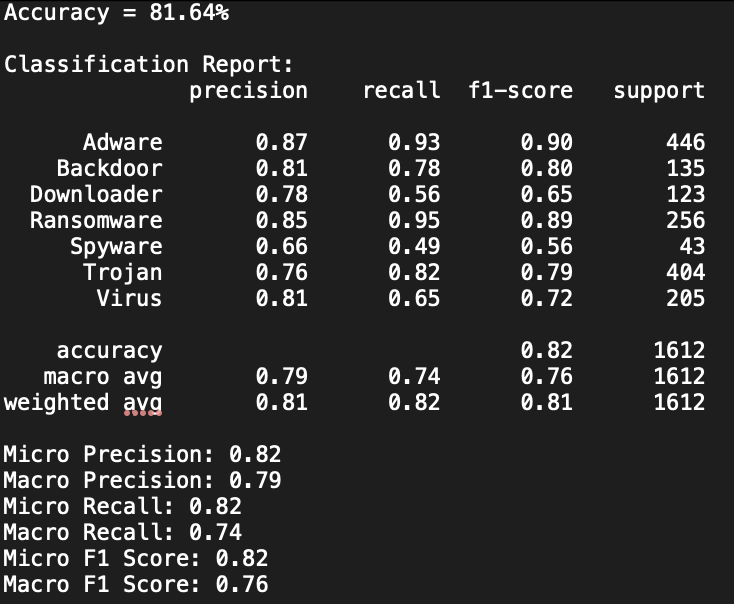
\includegraphics[width=0.8\linewidth]{images/evaluation.png}
        \label{fig:cnn_architecture}
\end{figure}
\captionof{figure}{Metriche di valutazione della rete neurale convoluzionale (CNN) utilizzata}

\subsection{Matrice di Confusione}
La matrice di confusione fornisce un'analisi visiva dettagliata delle prestazioni del modello. Mostra le predizioni corrette e gli errori di classificazione per ciascuna classe in una tabella. Ogni riga rappresenta i valori reali e ogni colonna le predizioni del modello, evidenziando i seguenti elementi:
\begin{itemize}
    \item \textbf{Vero Positivo (TP)}: Campioni correttamente predetti come appartenenti a una classe.
    \item \textbf{Falso Positivo (FP)}: Campioni che sono stati erroneamente predetti come appartenenti a una classe.
    \item \textbf{Falso Negativo (FN)}: Campioni che appartenevano a una classe ma non sono stati riconosciuti come tali.
    \item \textbf{Vero Negativo (TN)}: Campioni correttamente identificati come non appartenenti a una classe.
\end{itemize}

Dalla tabella \ref{tab:confusion_matrix} emerge che le classi "Adware" e "Ransomware" sono quelle classificate con la maggiore accuratezza, con elevati valori di veri positivi (TP) e bassi valori di falsi negativi (FN). Tuttavia, per alcune classi come "Spyware" e "Downloader", si osserva un maggior numero di errori, evidenziando la difficoltà del modello nel distinguere alcune classi che possono avere caratteristiche simili.
\begin{table}[h]
    \centering
    \begin{tabular}{|c|c|c|c|c|c|c|}
    \hline
    \textbf{Adware} & \textbf{Backdoor} & \textbf{Downloader} & \textbf{Ransomware} & \textbf{Spyware} & \textbf{Trojan} & \textbf{Virus} \\
    \hline
    415 & 1  & 3  & 0  & 2  & 15 & 10 \\
    \hline
    4   & 105 & 2  & 3  & 1  & 20 & 0  \\
    \hline
    7   & 10  & 69 & 6  & 1  & 27 & 3  \\
    \hline
    0   & 0   & 3  & 242 & 1  & 10 & 0  \\
    \hline
    1   & 1   & 3  & 3   & 21 & 14 & 0  \\
    \hline
    13  & 8   & 5  & 25  & 4  & 331 & 18 \\
    \hline
    38  & 4   & 4  & 7   & 2  & 17 & 133 \\
    \hline
    \end{tabular}
    \caption{Matrice di Confusione}
    \label{tab:confusion_matrix}
\end{table}
    
\newpage
\section{Generative Adversarial Network}
%TODO Migliorare questa parte
Generatore genera l'immagine. La blackbox (ovvero mio modello CNN pre-addestrato) fa una predizione riguardante la tipologia di famiglia a cui appartiene quella determinata immagine. SE la predizione è giusta, allora il generatore procede nell'inserire in po' di rumore all'interno della stessa immagine. Questo continua fino a che la blackbox non viene illusa. Fa questa csoa per un fracco di volte.
\subsection{Architettura}
\begin{figure}[ht]
    \centering
        \centering
        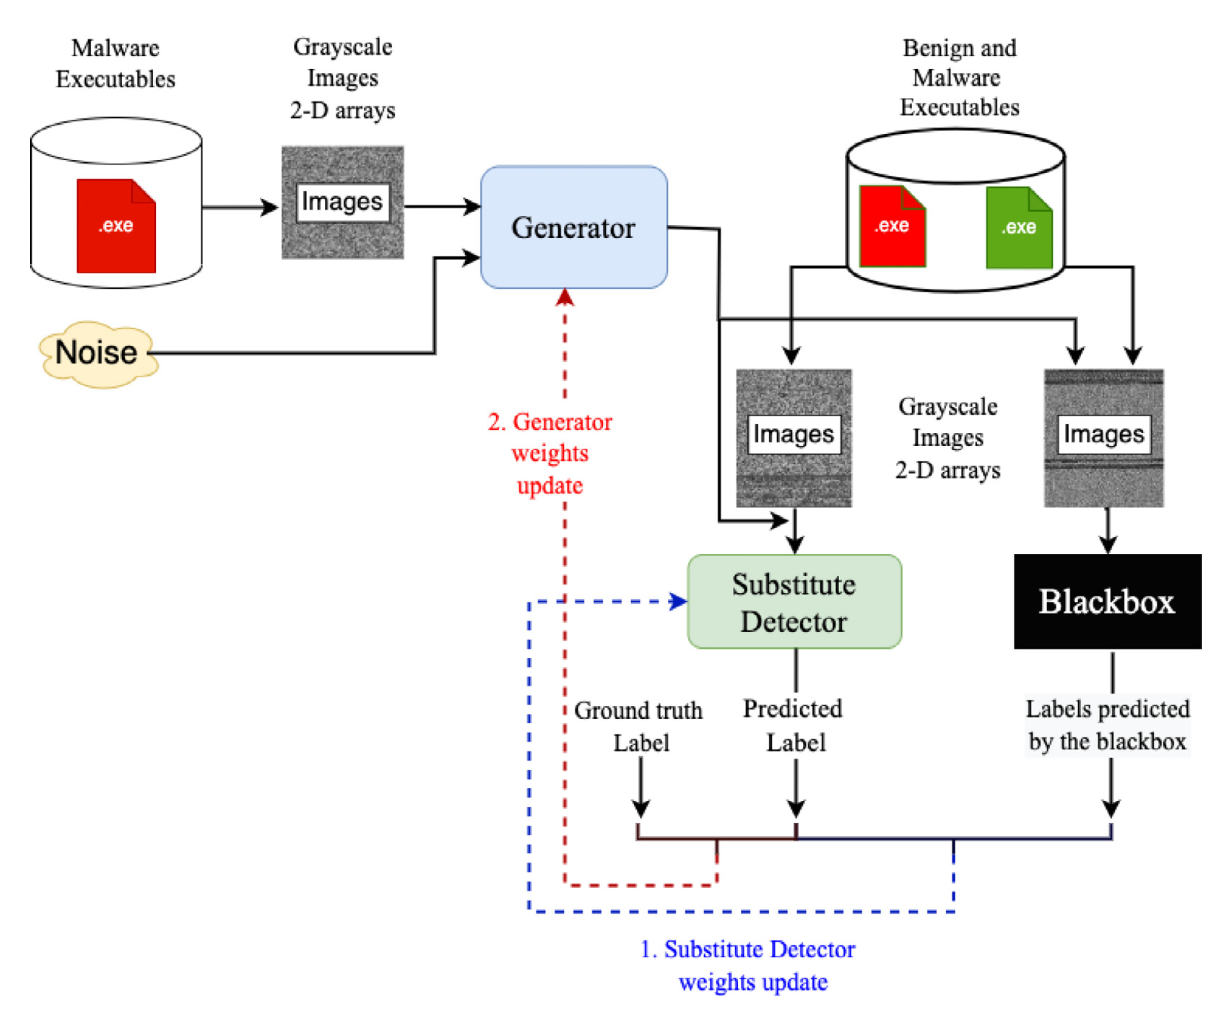
\includegraphics[width=0.8\linewidth]{images/GAN_architecture.png}
        \label{fig:gan_architecture}
\end{figure}
\captionof{figure}{Architettura della Generative Adversarial Network (GAN) utilizzata}

\subsection{Generatore}
\subsubsection{Struttura}
\subsubsection{Funzionamento}
\subsubsection{Processo di addestramento}

\subsection{Discriminatore}
\subsubsection{Struttura}
\subsubsection{Funzionamento}
\subsubsection{Processo di addestramento}

\subsection{Applicazioni}
Le Generative Adversarial Networks (GAN) rappresentano una delle architetture di machine learning più innovative e potenti degli ultimi anni. Combinando due reti neurali, il generatore e il discriminatore, le GAN sono state applicate con successo in numerosi ambiti, tra cui la generazione di immagini, la sintesi del linguaggio e, più recentemente, nella rilevazione e creazione di malware. Sebbene le GAN siano principalmente note per la loro capacità di generare dati sintetici altamente realistici, il loro impiego in cybersecurity, e in particolare nella manipolazione e generazione di malware, sta acquisendo sempre più attenzione.

\subsubsection{Generazione di Malware per l'Analisi e la Rilevazione}

Una delle applicazioni emergenti delle GAN nel contesto del malware è la generazione di malware sintetico. Le GAN possono essere utilizzate per creare nuovi campioni di malware che replicano le caratteristiche delle minacce informatiche esistenti. Questo approccio consente di arricchire i dataset di malware, che sono spesso sbilanciati o insufficienti, con nuovi esempi che possono essere utilizzati per addestrare modelli di rilevazione più robusti e accurati. Generando malware sintetico, è possibile simulare scenari di attacco reali senza compromettere la sicurezza, permettendo agli esperti di cybersecurity di testare e affinare i sistemi di difesa.

Le GAN si distinguono particolarmente nella creazione di varianti di malware che mantengono le stesse caratteristiche funzionali ma con differenze sufficienti da eludere i sistemi di rilevamento tradizionali. Questi modelli generativi sono in grado di apprendere le modalità di evasione dei rilevatori, come quelli basati su firma o comportamentali, e creare malware che possiede capacità di auto-modifica, mimetizzandosi meglio nei sistemi di sicurezza.

\subsubsection{Miglioramento dei Sistemi di Rilevamento}

Un'altra area cruciale in cui le GAN stanno trovando applicazione è nel miglioramento dei sistemi di rilevamento del malware. Tradizionalmente, i sistemi di rilevamento si basano su tecniche come l'analisi delle firme o l'analisi comportamentale. Tuttavia, queste tecniche spesso falliscono quando il malware si evolve rapidamente, specialmente nei casi in cui il codice cambia per sfuggire ai sistemi di sicurezza. Le GAN, in questo caso, possono essere utilizzate per addestrare modelli di rilevamento più robusti, generando nuovi campioni di malware che i sistemi di difesa non hanno mai visto prima.

L'approccio di adversarial training (addestramento avversario) con le GAN è particolarmente promettente: durante l'addestramento, il generatore crea malware sintetico che viene utilizzato per ingannare il discriminatore, che cerca di classificarlo come malware o come software legittimo. Questo processo aiuta a migliorare la capacità del modello di rilevare anche minacce sconosciute e mai viste, aumentando l'efficacia dei sistemi di sicurezza.

\subsubsection{Evasione e Attacchi Avanzati}
Le GAN sono anche utilizzate in ambito offensivo per creare attacchi adversariali mirati, cioè malware progettato per aggirare specifici sistemi di difesa. Utilizzando la capacità delle GAN di generare nuovi dati in modo iterativo e migliorato, gli attaccanti possono creare malware che riesce a bypassare i sistemi di rilevazione basati su machine learning. In questo caso, il generatore produce varianti del malware che cercano deliberatamente di eludere i filtri di rilevamento, mentre il discriminatore aiuta a ottimizzare il processo di evasione, rendendo l'attacco sempre più difficile da identificare.

\subsection{Tipologie}
Nel contesto delle Generative Adversarial Networks (GAN), esistono numerosi tipi e varianti progettati per migliorare le prestazioni in compiti specifici come la generazione di immagini, il miglioramento della qualità delle immagini, o l'adattamento ai dati di input. Di seguito vengono descritti alcuni dei modelli più rilevanti: MiGAN, MalGAN, Xception, e InceptionNet.

\subsubsection{MiGAN (Malware Image Generative Adversarial Network)}
MiGAN è una variante delle GAN utilizzata per la generazione di immagini di malware. È particolarmente utile nel campo della cybersecurity per migliorare la rilevazione e la generazione di nuove varianti di malware, e si concentra sulla sintesi di immagini di malware che imitano le caratteristiche visive delle minacce esistenti ma con l'intento di eludere i sistemi di rilevamento.

\subsubsubsection{Architettura di MiGAN}
L'architettura di MiGAN è composta da un generatore e da un discriminatore, simile a una GAN tradizionale, ma progettata per gestire immagini di malware. La struttura del modello è la seguente:
\begin{itemize}
    \item \textbf{Generatore (G)}: Il generatore crea immagini di malware sintetiche a partire da un vettore di rumore casuale, utilizzando convoluzioni trasposte e batch normalization. La rete è composta da diversi strati di convoluzione, ognuno dei quali espande la dimensione dell'immagine, partendo da un basso livello di dettaglio a uno più alto. 
    \begin{itemize}
        \item Strato di \texttt{Dense}: Per iniziare con un vettore di rumore.
        \item Strato \texttt{Reshape}: Per adattare l'output del \texttt{Dense} in una forma adatta alla convoluzione.
        \item Strati di \texttt{Conv2DTranspose}: Convoluzioni trasposte per ingrandire l'immagine.
        \item \texttt{BatchNormalization}: Per migliorare la stabilità dell'apprendimento.
        \item Funzione di attivazione \texttt{ReLU}: Per la maggior parte degli strati.
        \item \texttt{Tanh}: Per l'output, che restituisce valori tra -1 e 1, tipici delle immagini.
    \end{itemize}
    \item \textbf{Discriminatore (D)}: Il discriminatore è una rete neurale convoluzionale che cerca di distinguere tra immagini di malware reali e quelle sintetiche. Essa utilizza convoluzioni per ridurre progressivamente la dimensione spaziale dell'immagine, utilizzando anche \texttt{LeakyReLU} come funzione di attivazione.
    \begin{itemize}
        \item Strati \texttt{Conv2D}: Convoluzioni per l'estrazione delle caratteristiche.
        \item \texttt{LeakyReLU}: Per prevenire i vanishing gradients.
        \item \texttt{Dropout}: Per evitare overfitting.
        \item \texttt{Flatten}: Per appiattire l'immagine.
        \item \texttt{Dense}: Per ottenere una singola probabilità tra 0 (reale) e 1 (falsa).
    \end{itemize}
\end{itemize}
Questa architettura consente di generare nuove varianti di malware che possono essere utilizzate per allenare modelli di rilevamento più robusti.

\subsubsection{MalGAN (Malware Generative Adversarial Network)}

MalGAN è un'architettura GAN progettata per eludere i sistemi di rilevamento del malware esistenti. A differenza di MiGAN, che genera immagini di malware, MalGAN si concentra sulla creazione di varianti che possano bypassare i modelli di machine learning tradizionali.

\subsubsubsection{Architettura di MalGAN}
MalGAN si basa su un'architettura GAN simile a quella di MiGAN, ma con un focus sull'ottimizzazione delle capacità di evasione. In particolare, MalGAN integra un meccanismo di \textit{adversarial training} per creare esempi di malware che sono difficili da rilevare dai modelli di sicurezza.
\begin{itemize}
    \item \textbf{Generatore (G)}: Crea varianti di malware per ingannare il discriminatore. Il generatore è composto da:
    \begin{itemize}
        \item Strato \texttt{Dense} seguito da \texttt{Reshape}.
        \item Strati \texttt{Conv2DTranspose} per amplificare la dimensione dell'immagine.
        \item Normalizzazione e \texttt{ReLU} per attivazioni.
    \end{itemize}
    \item \textbf{Discriminatore (D)}: È un classificatore binario che distingue tra malware reale e generato. Utilizza:
    \begin{itemize}
        \item Strati \texttt{Conv2D} con \texttt{LeakyReLU}.
        \item \texttt{Dropout} per migliorare la generalizzazione.
        \item Funzione di attivazione \texttt{Sigmoid} per la probabilità di autenticità.
    \end{itemize}
\end{itemize}
Il modello di MalGAN è addestrato su varianti di malware esistenti, cercando di ottimizzare la sua capacità di generare malware che può sfuggire ai rilevatori.

\subsubsection{Xception (Extreme Inception)}

Xception è una rete neurale convoluzionale basata su una versione avanzata di Inception, ed è progettata per migliorare l'efficienza computazionale attraverso l'uso di convoluzioni separabili in profondità.

\subsubsubsection{Architettura di Xception}
Xception si distingue dall'architettura Inception tradizionale, poiché utilizza convoluzioni separabili in profondità, che separano le convoluzioni spaziali e di canale. Questo approccio migliora l'efficienza computazionale e consente una maggiore espressione del modello.
\begin{itemize}
    \item \textbf{Convoluzioni separabili in profondità}: Separano le operazioni di convoluzione in due passaggi: uno per ciascun canale e uno per la combinazione dei canali. Questo riduce il numero di parametri e aumenta l'efficienza.
    \item Strati \texttt{Conv2D}: Applicati ai dati separatamente per ciascun canale.
    \item Strati \texttt{MaxPooling2D}: Per ridurre le dimensioni spaziali.
    \item \texttt{GlobalAveragePooling2D}: Utilizzato per ridurre le dimensioni della feature map, migliorando la generalizzazione.
    \item Strati \texttt{Dense}: Per la classificazione finale con \texttt{Softmax}.
\end{itemize}
Questa architettura è ampiamente utilizzata in compiti di visione artificiale, inclusa la classificazione delle immagini.

\subsubsection{InceptionNet}

InceptionNet è una rete neurale convoluzionale progettata per essere altamente efficiente, utilizzando un approccio modulare che combina convoluzioni di diverse dimensioni e pooling.

\subsubsubsection{Architettura di InceptionNet}
InceptionNet utilizza moduli Inception che permettono di eseguire convoluzioni di diverse dimensioni, migliorando la capacità della rete di apprendere a più scale.
\begin{itemize}
    \item \textbf{Inception Module}: Ogni modulo esegue convoluzioni di diverse dimensioni (1x1, 3x3, 5x5) e le concatena, permettendo alla rete di esplorare diverse scale di caratteristiche.
    \item Strati \texttt{Conv2D}: Eseguiti con kernel di dimensioni diverse all'interno dello stesso modulo.
    \item \texttt{Pooling Layers}: Combinazione di max-pooling e average-pooling.
    \item \texttt{1x1 Convoluzioni}: Utilizzate per ridurre la dimensionalità, migliorando l'efficienza computazionale.
    \item Strati \texttt{Dense}: Per la classificazione finale.
    \item \texttt{Softmax}: Per la normalizzazione delle probabilità.
\end{itemize}
Questa architettura è stata utilizzata con successo in competizioni di riconoscimento delle immagini e classificazione di oggetti, come il ImageNet Challenge.

\subsubsection{Problematiche attuali}
\label{Problema}
Il dataset era troppo sbilanciato. Questo ha portato a una minore precisione e accuratezza del modello. Inoltre, il dataset era troppo piccolo per garantire una rappresentazione accurata di tutte le classi di malware. Questo ha portato a una minore capacità del modello di generalizzare e rilevare nuove varianti di malware. Infine, l'architettura del modello potrebbe essere migliorata per ottenere prestazioni migliori, ad esempio utilizzando un'architettura più avanzata come Xception o InceptionNet.
Essendo un dataset molto piccolo, la classificazione è stata effettuata mediante superfamiglia, non singola famiglia. Questo ha portato a una minore precisione e accuratezza del modello, poiché le superfamiglie contengono molte classi diverse con caratteristiche simili.
Limitazioni della capacità della macchina su cui sono stati effettuati l'addestramento ed i test del modello. Questo ha portato a tempi di addestramento più lunghi e a una minore capacità di esplorare l'architettura del modello e ottimizzare i parametri.

\subsubsubsection{Miglioramenti}
Dataset meno sbilanciato, più accurato e più grande
Classificazione per singola famiglia e superfamiglia rende il modello più preciso nella rilevazione
Improvement dei layer del modello
